\documentclass[12pt,letterpaper]{article}
\usepackage{graphicx,textcomp}
\usepackage{natbib}
\usepackage{setspace}
\usepackage{fullpage}
\usepackage{color}
\usepackage[reqno]{amsmath}
\usepackage{amsthm}
\usepackage{fancyvrb}
\usepackage{amssymb,enumerate}
\usepackage[all]{xy}
\usepackage{endnotes}
\usepackage{lscape}
\newtheorem{com}{Comment}
\usepackage{float}
\usepackage{hyperref}
\newtheorem{lem} {Lemma}
\newtheorem{prop}{Proposition}
\newtheorem{thm}{Theorem}
\newtheorem{defn}{Definition}
\newtheorem{cor}{Corollary}
\newtheorem{obs}{Observation}
\usepackage[compact]{titlesec}
\usepackage{dcolumn}
\usepackage{tikz}
\usetikzlibrary{arrows}
\usepackage{multirow}
\usepackage{xcolor}
\newcolumntype{.}{D{.}{.}{-1}}
\newcolumntype{d}[1]{D{.}{.}{#1}}
\definecolor{light-gray}{gray}{0.65}
\usepackage{url}
\usepackage{listings}
\usepackage{color}

\definecolor{codegreen}{rgb}{0,0.6,0}
\definecolor{codegray}{rgb}{0.5,0.5,0.5}
\definecolor{codepurple}{rgb}{0.58,0,0.82}
\definecolor{backcolour}{rgb}{0.95,0.95,0.92}

\lstdefinestyle{mystyle}{
	backgroundcolor=\color{backcolour},   
	commentstyle=\color{codegreen},
	keywordstyle=\color{magenta},
	numberstyle=\tiny\color{codegray},
	stringstyle=\color{codepurple},
	basicstyle=\footnotesize,
	breakatwhitespace=false,         
	breaklines=true,                 
	captionpos=b,                    
	keepspaces=true,                 
	numbers=left,                    
	numbersep=5pt,                  
	showspaces=false,                
	showstringspaces=false,
	showtabs=false,                  
	tabsize=2
}
\lstset{style=mystyle}
\newcommand{\Sref}[1]{Section~\ref{#1}}
\newtheorem{hyp}{Hypothesis}

\title{QTM 200: Applied Regression Analysis- Problem Set 5}
\date{Due: March 4, 2020}
\author{Farris Sabir}

\begin{document}
	\maketitle
	
	\section*{Instructions}
	\begin{itemize}
		\item Please show your work! You may lose points by simply writing in the answer. If the problem requires you to execute commands in \texttt{R}, please include the code you used to get your answers. Please also include the \texttt{.R} file that contains your code. If you are not sure if work needs to be shown for a particular problem, please ask.
		\item Your homework should be submitted electronically on the course GitHub page in \texttt{.pdf} form.
		\item This problem set is due at the beginning of class on Wednesday, March 4, 2020. No late assignments will be accepted.
		\item Total available points for this homework is 100.
	\end{itemize}
	
		\vspace{.5cm}
	
\noindent  Using the \texttt{teengamb} dataset, fit a model with \texttt{gamble} as the response and the other variables as predictors. 

\vspace{.5cm}
\lstinputlisting[language=R, firstline=41, lastline=43]{PS5.R}  
\vspace{.5cm}
Answer the following questions:
\vspace{.5cm}
\begin{enumerate}[(a)]
	 \item Check the constant variance assumption for the errors by plotting the residuals versus the fitted values.
	 
	 \lstinputlisting[language=R, firstline=47, lastline=47]{PS5.R}  
	 
	 	\begin{figure}[h!]
	 	\caption{\footnotesize{Residuals vs. Fitted}}
	 	\vspace{.5cm}
	 	\centering
	 	\label{fig:residvfitted}
	 	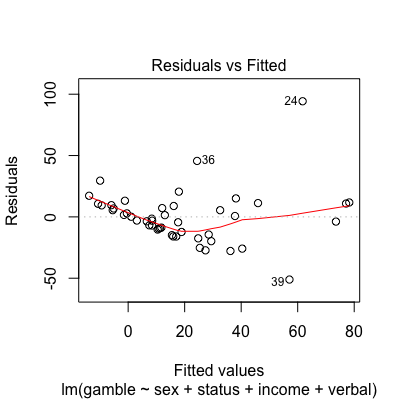
\includegraphics[width=1\textwidth]{./PS5_Graph_1.png}
	 \end{figure}	
 	
 	According to Figure 1, the constant variance assumption might be in question because the line of the in the graph is not completely straight, only slightly so. This may indicate variance may vary across different fitted values.
 
	 \vspace{1cm}
	 
	\item Check the normality assumption with a Q-Q plot of the studentized residuals. 
	
	\lstinputlisting[language=R, firstline=54, lastline=54]{PS5.R}
	
	\begin{figure}[h!]
	\caption{\footnotesize{Normal Q-Q}}
	\vspace{.5cm}
	\centering
	\label{fig:qqplot}
	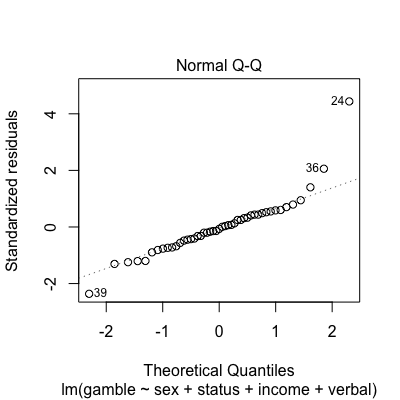
\includegraphics[width=1\textwidth]{./PS5_Graph_2.png}
	\end{figure}

	This Q-Q plot in Figure 2 supports the normality assumption because most values fall on the line. Values falling on the line indicate that variation in those x-values are normally distributed. More error occurs at the end, but that is expected, especially since there are less data for these end values.
	
	\vspace{.6cm}
	
	\item Check for large leverage points by plotting the $h$ values. 
	
	\lstinputlisting[language=R, firstline=61, lastline=64]{PS5.R}
	
	There are four points with high leverage using threshold of $\frac{2(k + 1)}{n}$, but not threshold of $\frac{3(k + 1)}{n}$ as shown in the Figure 3. 
	\begin{figure}[h!]
		\caption{\footnotesize{Hat Values Plot}}
		\vspace{.1cm}
		\centering
		\label{fig:hatplot}
		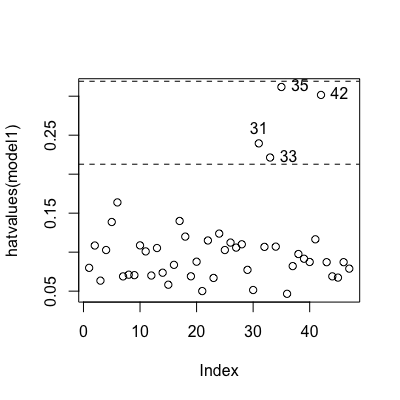
\includegraphics[width=1\textwidth]{./PS5_Graph_3.png}
	\end{figure}
	
	These points have the potential to greatly influence the fitted model:
	
	\lstinputlisting[language=R, firstline=67, lastline=67]{PS5.R}
	
	\begin{verbatim}
	sex status income verbal gamble
	31   0     18   12.0      2   88.0
	33   0     38   15.0      7   90.0
	35   0     28    1.5      1   14.1
	42   0     61   15.0      9   69.7
	\end{verbatim} 
	
	\vspace{.6cm}
	
	\item Check for outliers by running an \texttt{outlierTest}.
	
	\lstinputlisting[language=R, firstline=72, lastline=72]{PS5.R}
	
	\begin{verbatim}
		 			      	rstudent  		unadjusted p-value 		Bonferroni p
		24 	     6.016116         4.1041e-07   					1.9289e-05
	\end{verbatim} 
	
	Because the adjusted p-value for the largest studentized residual is less than 0.05, this 24th observation has an extreme residual or is an outlier.
	
	\vspace{.6cm}
	
	\item Check for influential points by creating a "Bubble plot" with the hat-values and studentized residuals.
	
	\lstinputlisting[language=R, firstline=78, lastline=83]{PS5.R}
	
	\begin{figure}[h!]
		\caption{\footnotesize{Bubble Plot}}
		\vspace{.1cm}
		\centering
		\label{fig:bubble}
		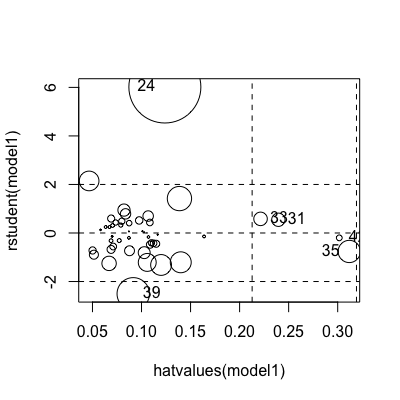
\includegraphics[width=1\textwidth]{./PS5_Graph_4.png}
	\end{figure}
	
	Figure 4 helps track which points possibly and actually are influential.
	
	The same four points from part (c) have high leverage under threshold of $\frac{2(k + 1)}{n}$, but not threshold of $\frac{3(k + 1)}{n}$. 
	
	Two points have some of the largest regression residuals, the 24th and 39th observation.

		\begin{verbatim}
	   sex status income verbal gamble
		24   0     27     10      4    156
		39   0     51     10      6      6
		\end{verbatim} 
	
	The 24th observation likely has the largest influence on the model. It has a large regression residual, as verified by part d, and large Cook's distance.
	
	% \item N/A.
\end{enumerate}

\end{document}
